\documentclass[onecolumn]{article} % Two-column layout

% Packages
\usepackage[utf8]{inputenc} % Encoding
\usepackage{graphicx}       % For including images
\usepackage{amsmath}        % For mathematical equations
\usepackage{cite}           % For citations
\usepackage{geometry}       % Adjust margins
\geometry{margin=1in}      % Set margins

% Document
\begin{document}

% Title
\title{\textbf{Invisibility Cloak}}
\author{Your Name}
\date{\today} % Sets date to current date
\maketitle


% Main Content
\section{Introduction}

Modern technological advancements in augmented reality, computer vision, and real-time image processing have opened doors to numerous innovative projects. One particularly fascinating concept is the invisibility cloak—a system that creates the effect of a person or object disappearing by merging into their surroundings. This concept draws inspiration from *Harry Potter*, where magical cloaks enable characters to vanish from sight, and translates it into a technological application using advanced image processing.

The principle of achieving this invisibility effect relies on detecting a defined color range in a live video feed, masking it, and substituting it with a static or real-time background. This allows individuals wearing garments of a specific color (e.g., green, red, or another identifiable hue) to become effectively “invisible” by blending seamlessly into the environment. To achieve this effect, real-time image processing techniques, such as color filtering, background subtraction, and morphological transformations, must be utilized to maintain smooth transitions and consistent performance.

The primary goal of this project is to implement a real-time prototype of this effect using cutting-edge video processing methods. The system intends to address challenges such as lighting variations, environmental interference, and processing delays to ensure effective detection and elimination of undesired visual artifacts. Inspired by *Harry Potter* and grounded in computer vision techniques, this project seeks to bridge imagination and innovation by turning the invisibility effect into a functional technological reality.

\vspace{0.5cm}

\section{Problem Statement}

Despite the rapid progress in augmented reality and machine learning, achieving a real-time invisibility effect with low latency presents significant challenges. Many real-time video processing methods are hindered by delays, inaccuracies, or environmental inconsistencies, particularly under varying lighting or changing perspectives.

The challenges this project aims to address are as follows:

\begin{itemize}
    \item \textbf{Real-time Detection and Masking:} Developing a system capable of dynamically identifying and masking a specific color range in real time with minimal latency.
    \item \textbf{Noise Elimination:} Managing variations in lighting conditions, camera noise, and environmental changes that can affect the accuracy of the detection process.
    \item \textbf{Seamless Background Integration:} Ensuring the detected area is blended smoothly into the background without visible artifacts to maintain the illusion of invisibility.
\end{itemize}

To address these challenges, the proposed solution employs color-based cloaking mechanisms through HSV (Hue, Saturation, and Value) filtering, morphological image processing, and real-time background subtraction. This approach allows individuals wearing garments of a specific color to achieve the visual effect of disappearing by dynamically replacing their presence with the corresponding real-time background.

This project highlights how real-time video processing and computer vision can transform interactive effects into practical applications, offering a tangible example of augmented reality's potential.

\section{Works on Which the Invisibility Cloak Program is Based}

The concept of the invisibility cloak effect is rooted in previous research and technological developments spanning fields such as computer vision, augmented reality (AR), and image processing. This section outlines the primary areas of study and technological advancements that have influenced the development of the invisibility cloak effect in this project:

\subsection{Augmented Reality and Visual Cloaking}
The idea of creating visual effects to make objects or individuals disappear has its origins in augmented reality (AR) research. AR explores the manipulation of real-time video streams and backgrounds to create immersive and interactive visual effects. It does so by overlaying digital information onto live video feeds, forming the basis for interactive invisibility effects.

\subsection{Background Subtraction}
Background subtraction is a key area of research in real-time video analysis. It focuses on identifying moving objects or changes by dynamically comparing live video streams against static or changing backgrounds. Insights from this research have contributed to methods for detecting regions of interest and forming the backbone of real-time invisibility effects.

\begin{figure}[h!]
    \centering
    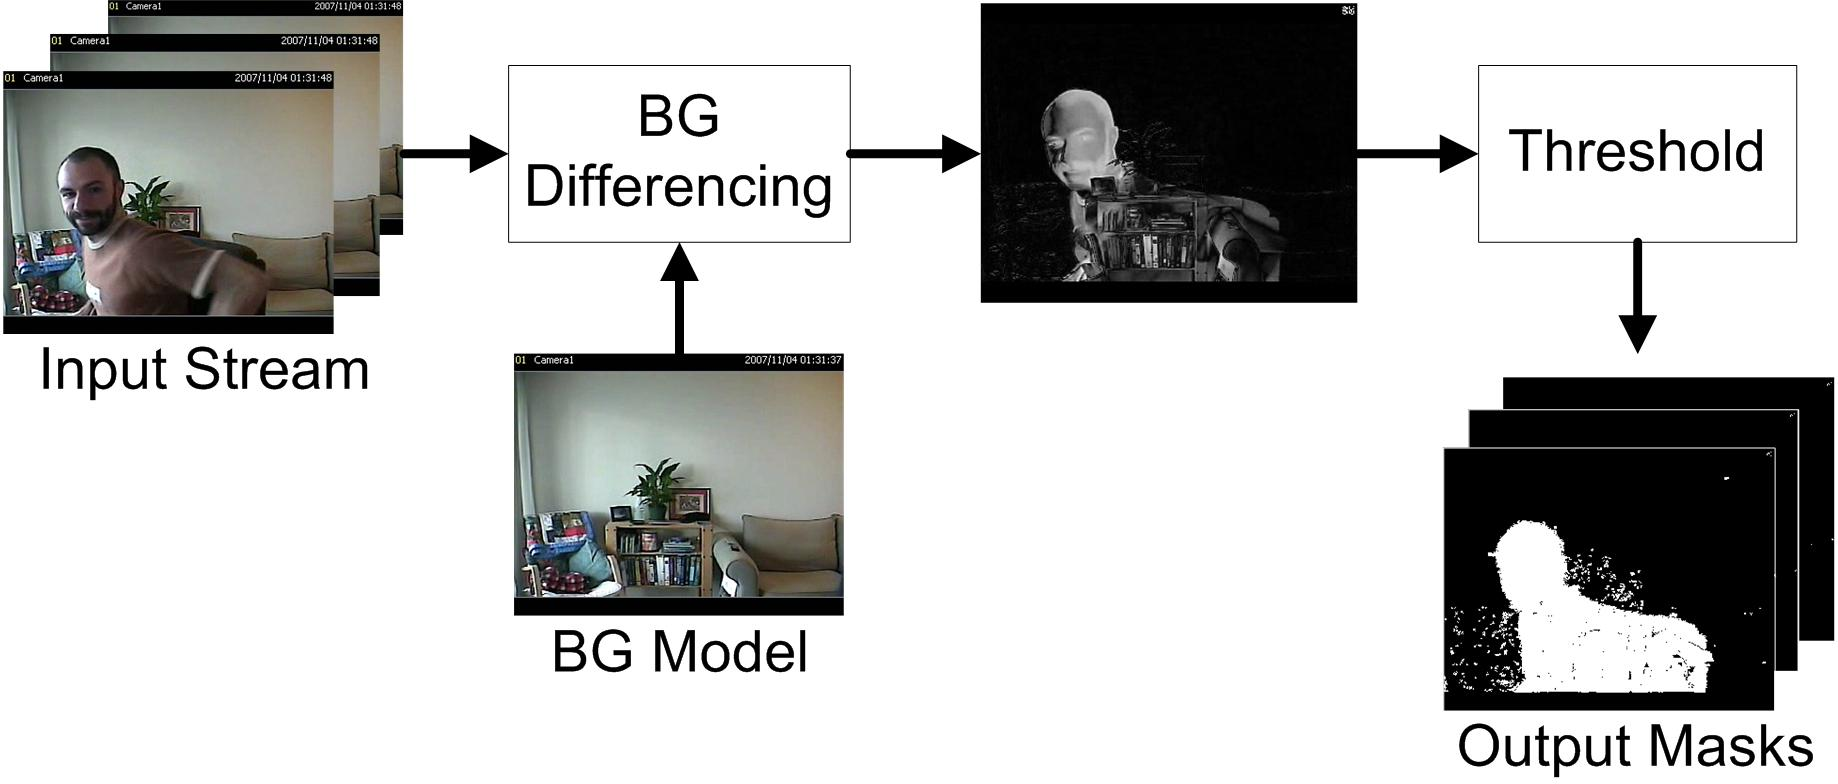
\includegraphics[width=0.45\textwidth]{Media\FrameDifferencing.jpg}
    \caption{Background subtraction using frame differencing techniques.}
    \label{fig:background_subtraction}
\end{figure}

\subsection{HSV Color Space Analysis}
The transition from RGB (Red, Green, Blue) color analysis to HSV (Hue, Saturation, and Value) color analysis represents an important milestone in real-time video analysis. HSV-based color detection allows for robust recognition of colors regardless of variations in lighting conditions or brightness, making it a vital component of reliable real-time image processing systems.

\begin{figure}[h!]
    \centering
    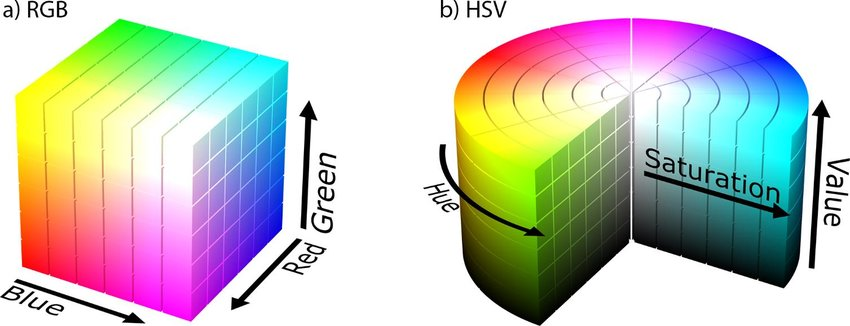
\includegraphics[width=0.45\textwidth]{Media\HSV.png}
    \caption{Visualization of HSV color space analysis in dynamic lighting conditions.}
    \label{fig:hsv_analysis}
\end{figure}

\subsection{Machine Learning Approaches for Real-Time Video Processing}
Machine learning and computer vision research have paved the way for adaptive and real-time analysis in augmented reality and video processing systems. These methodologies have enabled advanced detection mechanisms, allowing real-time analysis, detection of objects, and manipulation of video streams under varying environmental conditions.

\subsection{Visualization Effects Inspired by Fictional Concepts}
The idea of visual cloaking has been inspired by representations from science fiction, most notably in works like *Harry Potter*. Although fictional, these concepts sparked technological investigations into creating real-world invisibility effects. Researchers have taken inspiration from these ideas, combining computational methods with AR research to explore how similar effects can be achieved through real-time image processing.

\begin{figure}[h!]
    \centering
    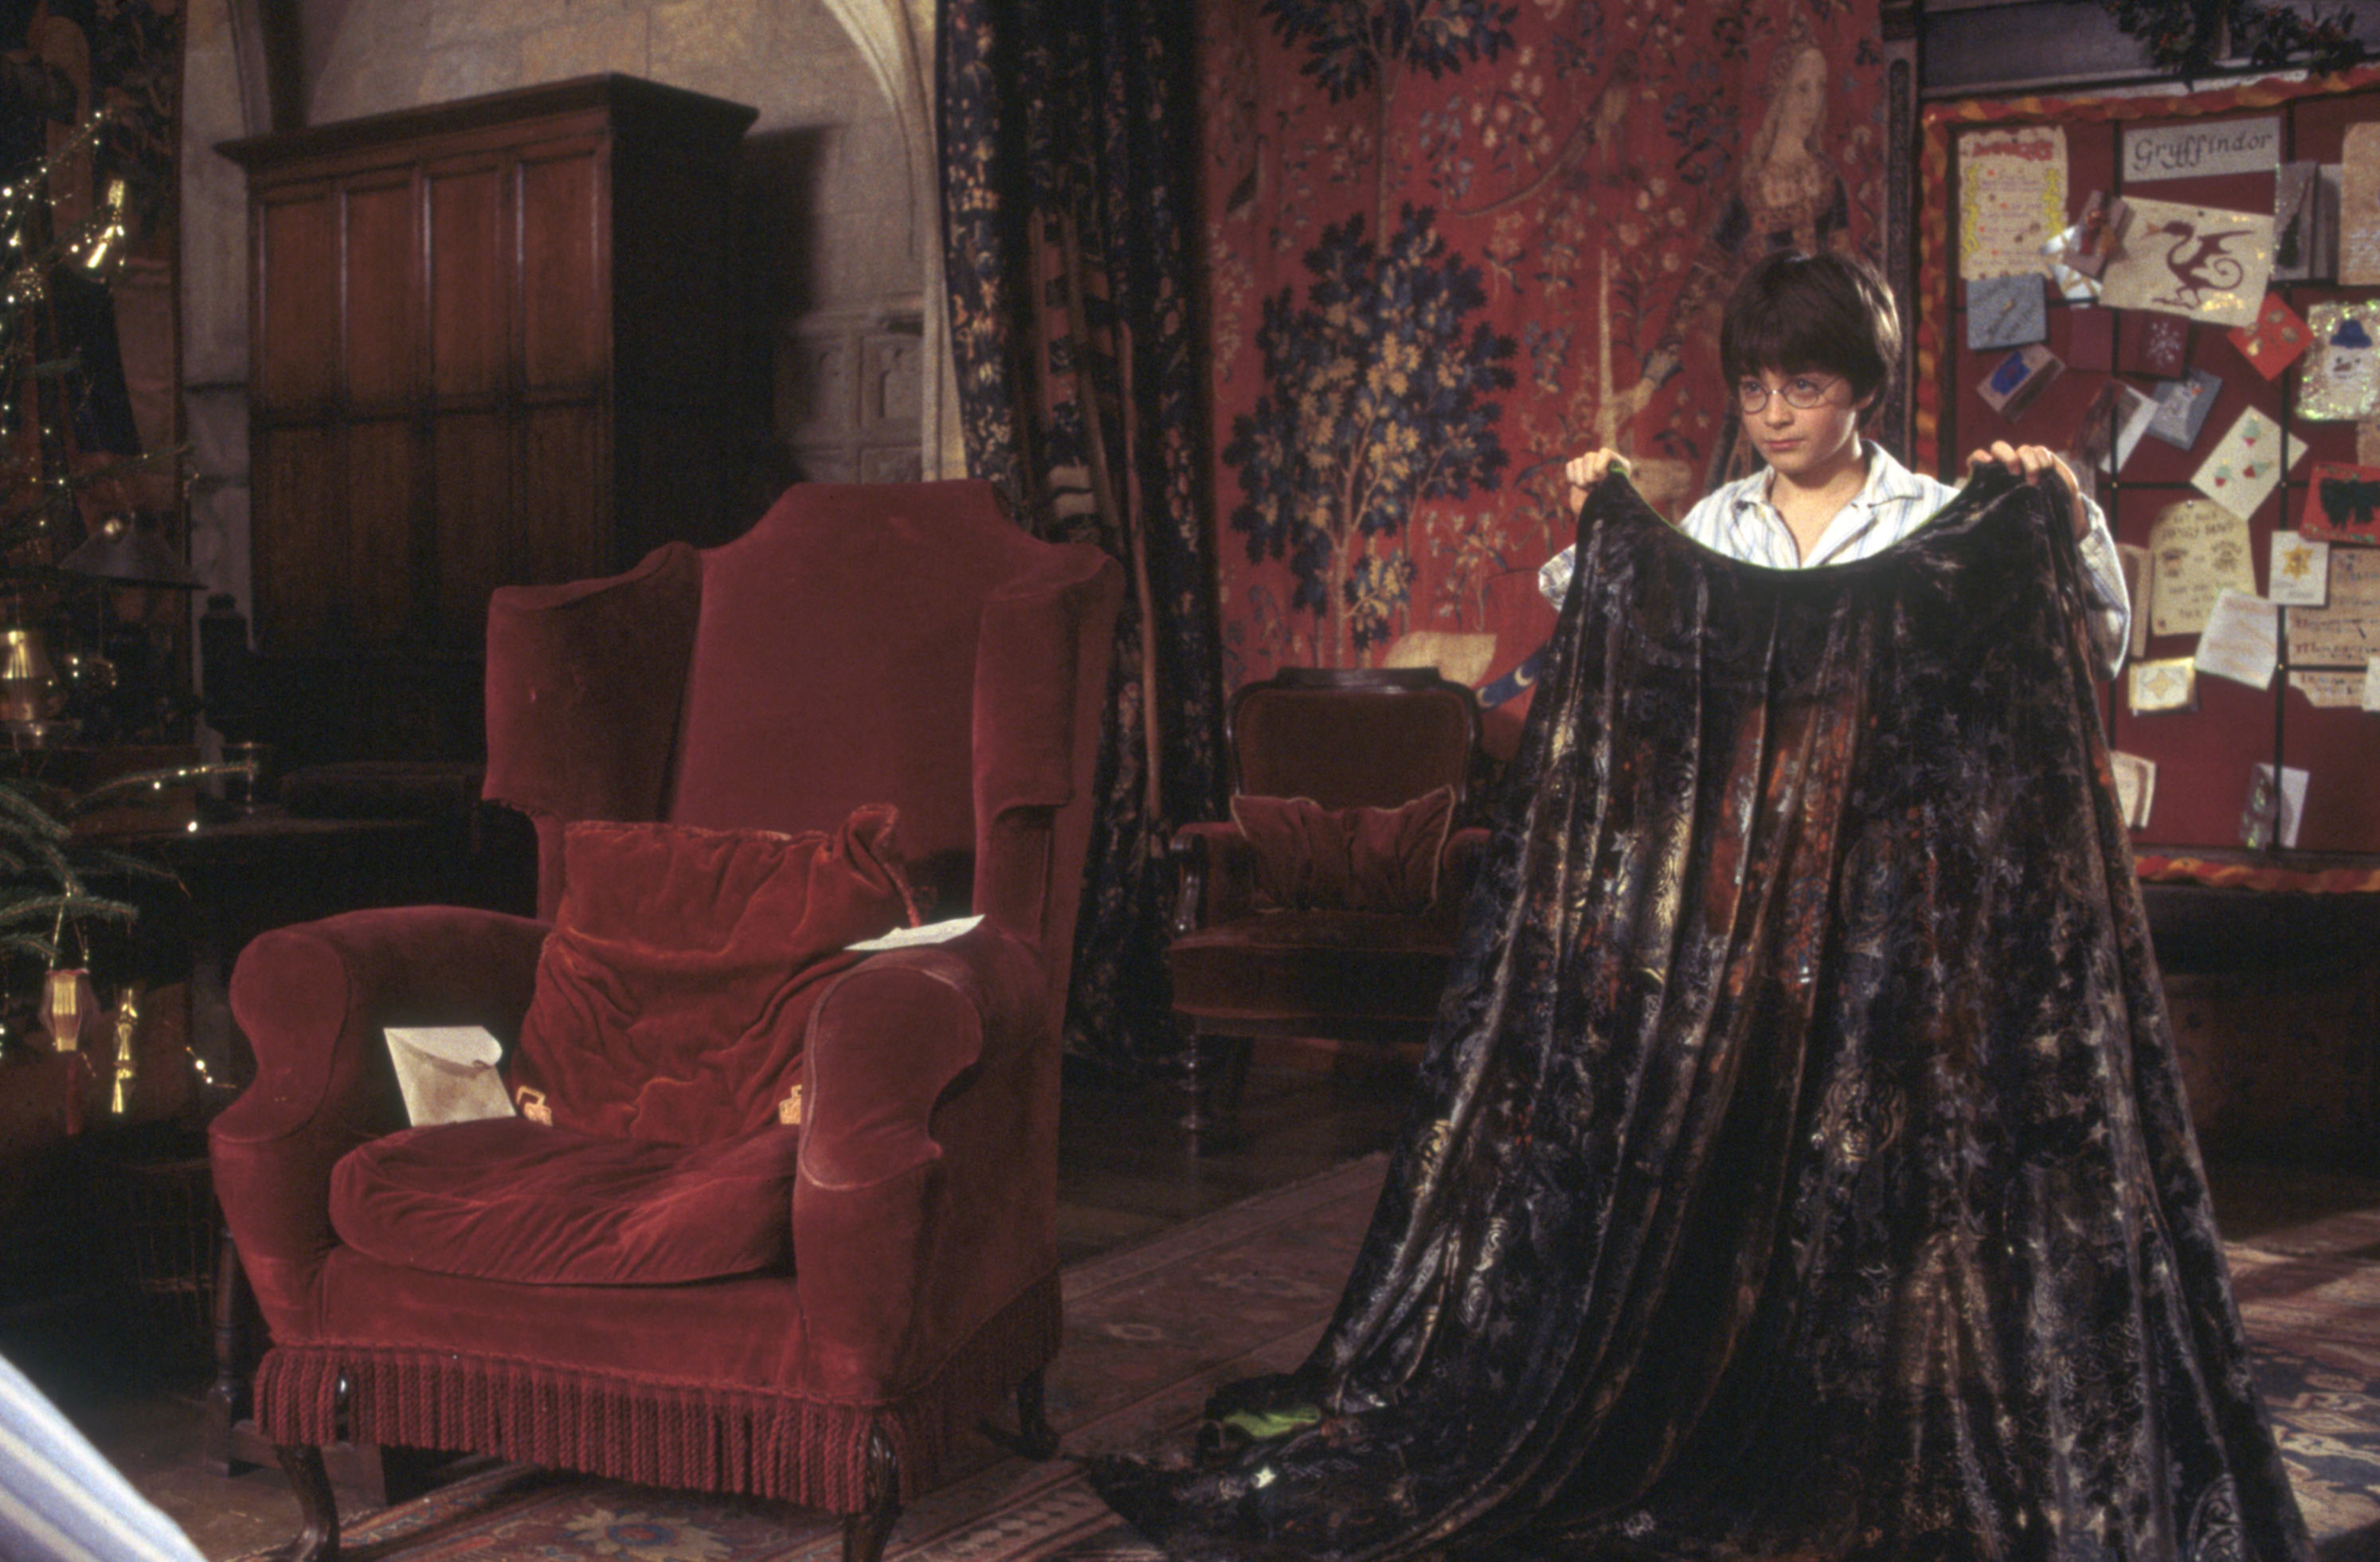
\includegraphics[width=0.45\textwidth]{Media\harry_potter.jpg}
    \caption{Harry Potter's iconic Invisibility Cloak.}
    \label{fig:hsv_analysis}
\end{figure}

\subsection{Noise Reduction and Real-Time Video Manipulation}
Video noise, inconsistent lighting, and varying environmental conditions present challenges for implementing seamless invisibility effects. Several studies have focused on using morphological image processing and filtering techniques to address these challenges. These methods ensure stable and reliable invisibility effects by minimizing noise and compensating for environmental fluctuations.

The integration of research insights from AR, HSV-based color detection, machine learning, background subtraction, and advanced image processing has laid the foundation for the invisibility cloak effect implemented in this project. These combined technological advancements and computational strategies form the conceptual underpinnings for creating a functional and real-time invisibility cloak effect.



\section{Methodology}
To achieve the invisibility cloak effect, several image processing methods and algorithms have been applied systematically. These methods involve real-time image manipulation techniques using computer vision libraries like OpenCV. The following steps describe the methods implemented.

\subsection{Pre-processing with Bilateral Filtering}

The initial step involves noise reduction while retaining the edges of objects within the frame. This is achieved using a bilateral filter, which smoothens the image while preserving edges.

The bilateral filter operates by considering both spatial proximity and color similarity when averaging pixel values. This preserves sharp edges and reduces artifacts that could affect the accuracy of subsequent image processing operations.

The filter applies weighted averaging to each pixel using these two Gaussian terms, ensuring that nearby pixels with similar intensities contribute more to the average.

The video frame is preprocessed using bilateral filtering before any further transformations. The OpenCV function `cv2.bilateralFilter()` is applied to the input frame with parameters for diameter \( d \), color standard deviation \( \sigma_\text{Color} \), and space standard deviation \( \sigma_\text{Space} \):

\[
\text{Filtered Frame} = \text{cv2.bilateralFilter}(\text{frame}, d=15, \sigma_\text{Color}=75, \sigma_\text{Space}=75)
\]

This step ensures that environmental noise and variations are minimized without distorting key visual features necessary for detecting colors during segmentation.

The figure below illustrates the effect of bilateral filtering applied to a raw video frame:

\begin{figure}[h!]
    \centering
    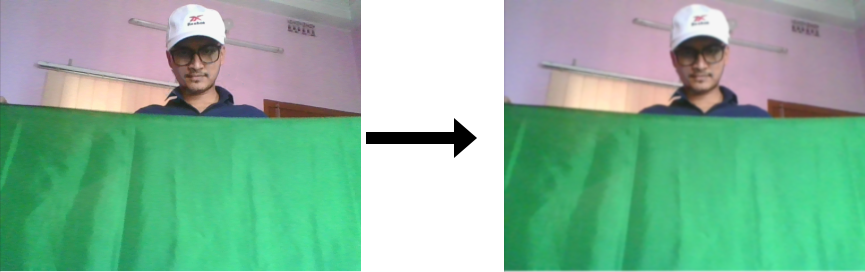
\includegraphics[width=0.8\textwidth]{Media\bilateral_filter.png}
    \caption{Effect of Bilateral Filtering on Input Frames. The noise is reduced while edge details are preserved.}
    \label{fig:bilateral_filtering}
\end{figure}

\subsection{Color Space Conversion to HSV}

Converting the input video frame from BGR to HSV color space is a fundamental step in achieving effective color detection under varying lighting conditions. The HSV (Hue, Saturation, Value) color space is particularly advantageous because it separates color information (hue and saturation) from brightness (value), making it robust to lighting changes.

The conversion involves transforming the input video frame into HSV format using computer vision libraries. HSV allows for more consistent detection of colors in real-world scenarios compared to the standard BGR color space.

The mathematical transformation used follows:

\[
\text{HSV} = \text{cv2.cvtColor}(\text{frame}, \text{cv2.COLOR_BGR2HSV})
\]

where `cv2.cvtColor` is applied to convert the color space of a given video frame from BGR (Blue, Green, Red) to HSV. This transformation ensures that color filtering remains consistent even when environmental factors, such as changes in brightness or lighting, affect the input video. HSV format helps segmentation based on color difference much more efficiently than BGR.

\begin{figure}[h!]
    \centering
    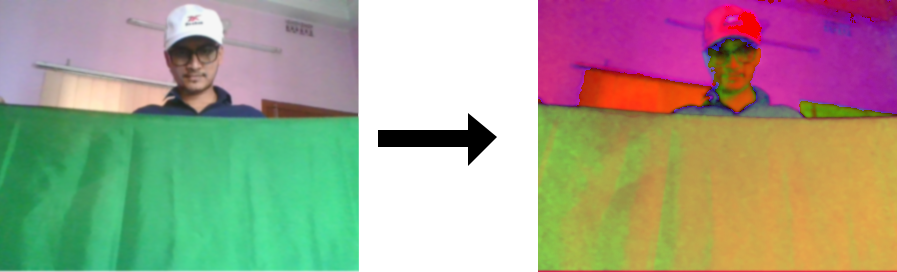
\includegraphics[width=0.8\textwidth]{Media\bgr_hsv.png}
    \caption{BGR to HSV Conversion.}
    \label{fig:BGR_HSV}
\end{figure}

\subsection{Applying Color Thresholding}

The function \texttt{cv2.inRange} is used to filter out specific colors from the converted HSV image. It creates a binary mask where pixels within a predefined range of hue, saturation, and value are set to 255 (white), while all other pixels are set to 0 (black). This step allows the system to focus on a specific color range that represents the cloak, enabling its detection and manipulation.

The process begins by first defining the lower and upper bounds for the hue, saturation, and value thresholds. These thresholds can be dynamically adjusted using sliders or pre-defined values. 
\[
\text{lower\_bound} = \text{np.array}([hue\_min, sat\_min, val\_min])
\]
\[
\text{upper\_bound} = \text{np.array}([hue\_max, 255, 255])
\]

The \texttt{cv2.inRange} function applies these thresholds to the HSV image to isolate the desired color range.

\[
\text{mask} = \text{cv2.inRange}(hsv, \text{lower\_bound}, \text{upper\_bound})
\]

Here:
- \texttt{hsv} is the transformed HSV image from the previous step,
- \texttt{lower\_bound} is the minimum range of hue, saturation, and value,
- \texttt{upper\_bound} is the maximum range of hue, saturation, and value.

The mask generated by \texttt{cv2.inRange} identifies regions in the video frame that correspond to the cloak's color. 

\begin{figure}[h!]
    \centering
    \includegraphics[width=0.8\textwidth]{Media\in range.png}
    \caption{Segmented Mask}
    \label{fig:Mask}
\end{figure}

\subsection{Morphological Operations: Dilation and Erosion for Mask Refinement}

Morphological operations, such as dilation and erosion, are critical in image processing for enhancing the mask's performance by reducing noise and filling gaps. These operations are applied to the binary mask obtained from \texttt{cv2.inRange}. The primary goal is to ensure that the mask smoothly detects the desired regions while eliminating small imperfections caused by lighting variations or environmental noise.

\textbf{Dilation and Erosion Overview:}  
Morphological operations work by modifying the structure of objects in a binary image using a defined kernel (a small matrix used to perform these operations). The two primary morphological operations involved are:

\begin{itemize}
    \item \textbf{Dilation:} Expands the white regions (value 255) in the mask, making the detected object area larger. It is effective for filling small gaps in the detection.
    \item \textbf{Erosion:} Shrinks the white regions, removing unwanted small regions of noise in the mask.
\end{itemize}

The sequence of operations involves:
\begin{enumerate}
    \item \textbf{Morphological Opening:} This is achieved by applying an erosion followed by a dilation. It removes noise by eliminating small white regions that do not match the desired shape of the target region.
    \item \textbf{Dilation:} After opening, additional dilation ensures that the final mask captures the entire cloak area with smooth boundaries.
\end{enumerate}

The applied morphological operations in the project can be mathematically expressed as follows:

\[
\text{kernel} = \text{np.ones}((3, 3), \text{np.uint8})
\]

\[
\text{mask} = \text{cv2.morphologyEx}(\text{mask}, \text{cv2.MORPH\_OPEN}, \text{kernel}, iterations=2)
\]

\[
\text{mask} = \text{cv2.morphologyEx}(\text{mask}, \text{cv2.MORPH\_DILATE}, \text{kernel}, iterations=1)
\]

\[
\text{mask} = \text{cv2.dilate}(\text{mask}, \text{kernel}, iterations=1)
\]

\begin{figure}[h!]
    \centering
    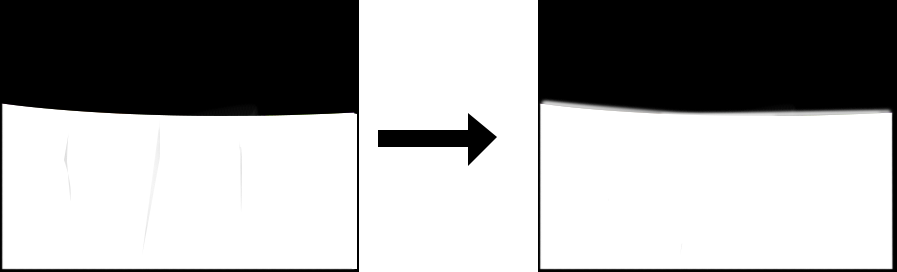
\includegraphics[width=0.8\textwidth]{Media\morpho.png}
    \caption{Applying Erosion and Dilation}
    \label{fig:Morpho}
\end{figure}
\textbf{Explanation of the Equations:}  
\begin{itemize}
    \item \textbf{cv2.MORPH\_OPEN:} This combines erosion followed by dilation to clean up small unwanted noise regions from the mask.
    \item \textbf{cv2.MORPH\_DILATE}\: Expands the detected region to ensure the cloak is fully captured without gaps.
    \item \textbf{kernel}\: A 3x3 matrix used to define the neighborhood of pixels for applying morphological changes.
\end{itemize}

These morphological operations collectively enhance the quality of the mask by ensuring it is less susceptible to environmental fluctuations, such as lighting changes or extraneous noise. After these operations, the mask becomes more robust and ensures smooth transitions when the cloak effect is applied, making the invisibility effect visually convincing.

\subsection{Application of Mask to Create the Cloaking Effect}

After obtaining and refining the binary mask through morphological operations, the next step involves applying the mask inversions and combining regions to simulate the invisibility effect. This section outlines how the mask was used mathematically and programmatically to manipulate the visibility of objects and backgrounds, creating the illusion of invisibility.

\textbf{Key Steps Involved:}  
The core idea is to selectively hide the cloak (or object wearing it) while simultaneously integrating the background into its visible region. This is achieved using bitwise operations, specifically \texttt{cv2.bitwise\_and}, and the mask's complement to simulate the invisibility effect.

\begin{enumerate}
    \item \textbf{Apply the Mask to the Background:}  
    Using a bitwise AND operation, the background is extracted only in regions where the mask indicates the cloak is absent. This operation ensures that when the cloak is in place, the background is shown seamlessly.

    \[
    \text{cloak} = \text{cv2.bitwise\_and}(\text{background}, \text{background}, \text{mask}).
    \]

    Here:
    \begin{itemize}
        \item \(\text{background}\): Represents the static or real-time background image.
        \item \(\text{mask}\): The binary mask that determines areas where the cloak should appear invisible.
    \end{itemize}

\begin{figure}[h!]
    \centering
    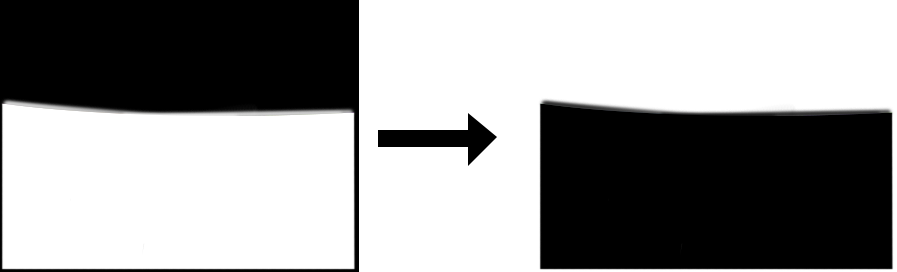
\includegraphics[width=0.8\textwidth]{Media\inverted mask.png}
    \caption{Inverted Mask}
    \label{fig:Inverted Mask}
\end{figure}

\begin{figure}[h!]
    \centering
    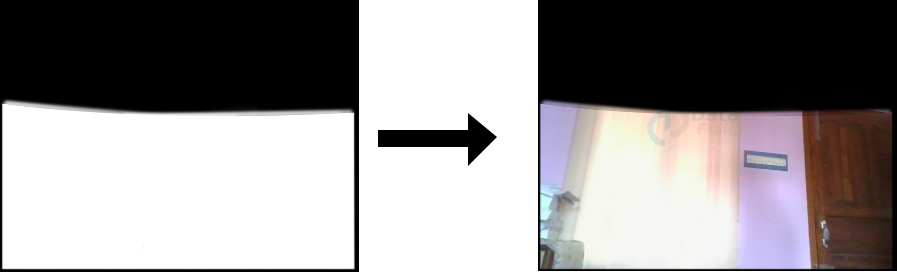
\includegraphics[width=0.8\textwidth]{Media\Masked.png}
    \caption{Applying Mask}
    \label{fig:Applying Mask}
\end{figure}

    \item \textbf{Extract the Non-Cloak Region from the Current Frame:}  
    The complement of the binary mask (\(\text{mask\_inv}\)) is used to isolate only the visible foreground regions from the current live video feed. This ensures that the non-cloak regions remain visible and unaffected by cloaking.

    \[
    \text{non\_cloak} = \text{cv2.bitwise\_and}(\text{frame}, \text{frame}, \text{mask\_inv}).
    \]

    Here:
    \begin{itemize}
        \item \(\text{mask\_inv}\): The inverted binary mask that highlights the visible areas of the frame.
    \end{itemize}

    \item \textbf{Combine the Two Regions:}  
    The `cv2.addWeighted` function is used to blend the cloak (background region) and non-cloak region into a single seamless image. This creates the final invisibility effect by showing the background in cloak regions and hiding the wearer selectively.

    \[
    \text{result} = \text{cv2.addWeighted}(\text{cloak}, 1, \text{non\_cloak}, 1, 0).
    \]

\begin{figure}[h!]
    \centering
    \includegraphics[width=0.8\textwidth]{Media\result.png}
    \caption{Result}
    \label{fig:Final Result}
\end{figure}

    This equation ensures that:
    \begin{itemize}
        \item The cloak region from the background is fully visible in places where the cloak effect should occur.
        \item The non-cloak region from the live video feed remains visible, preserving natural interactions with the environment.
    \end{itemize}
\end{enumerate}

\textbf{Visual Outcome:}  
The combination of these steps ensures a visually smooth transition, effectively making objects (or individuals) disappear as they blend into the real-time background using dynamic image manipulation.

This approach demonstrates how bitwise operations and mask inversions can be used innovatively to create an invisibility effect, seamlessly blending live video feeds and background information in real-time.


\section{Results}

The program successfully demonstrates the invisibility cloak effect by utilizing real-time video processing techniques, including background subtraction, HSV filtering, morphological operations, and mask manipulation. Upon implementation, the system was able to effectively identify a specific color range, mask it, and replace it with the background, achieving a visually convincing cloaking effect.

\begin{figure}[h!]
    \centering
    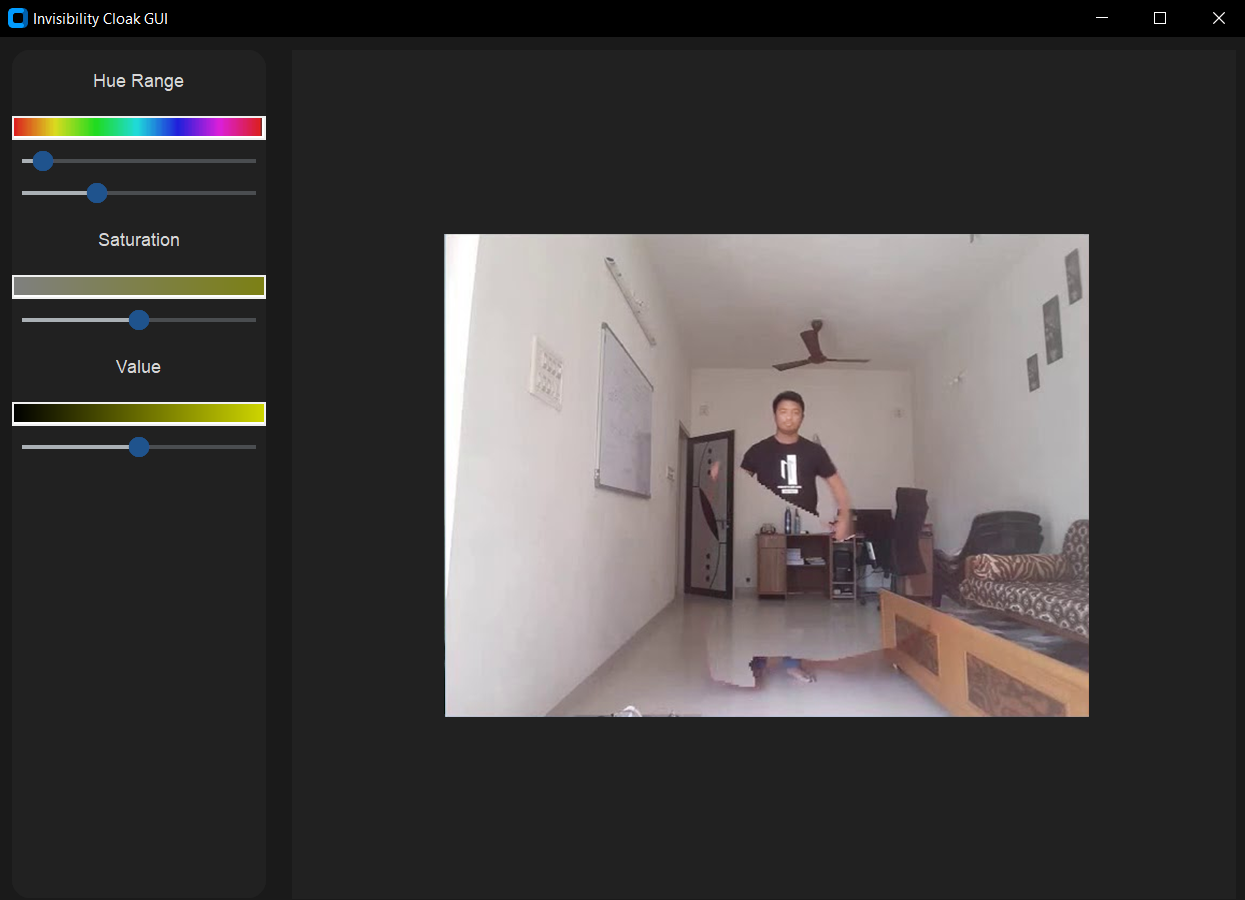
\includegraphics[width=0.8\textwidth]{gui.png}
    \caption{GUI}
    \label{fig:Graphical User Interface of the program}
\end{figure}

\subsection{Key Observations}

\begin{itemize}
    \item \textbf{Background Integration:} The system seamlessly blends the background with the cloak area, making it appear as though the object or person wearing the cloak is vanishing from view. This was achieved through the bitwise operations combining the live video feed and static background.
    
    \item \textbf{Dynamic Real-Time Processing:} The invisibility effect was processed in real-time with minimal delay, demonstrating the system's ability to handle live video input and video manipulation without perceptible lag.
    
    \item \textbf{Noise Management:} Morphological operations, such as dilation and erosion, proved effective in reducing visual noise from fluctuating light conditions and minor frame inconsistencies. This allowed for a stable and smooth transition between visible and invisible regions.
    
    \item \textbf{Color Detection Precision:} The use of HSV (Hue, Saturation, and Value) filtering ensured better accuracy in detecting the target cloak color under varying lighting conditions. This improved the system's robustness and ability to handle environmental variability.
    
    \item \textbf{Limitations Identified:} While the program performed well under controlled conditions, it faced some challenges with inconsistent lighting or highly dynamic backgrounds. Changes in lighting and shadows impacted the system's ability to maintain accurate masking, requiring further calibration for robustness.
\end{itemize}

\subsection{Conclusion}

The final results showcase the program's capability to replicate the invisibility effect as intended. This successful demonstration proves the feasibility of creating real-time augmented reality effects using advanced image processing methods. Future work can focus on improving system robustness, handling diverse lighting conditions, and further optimizing computational efficiency.




\end{document}
